%% ver4 (2026-11-17): Supplementary Information for main_v4.tex (to be submitted as one file, ESM_1.pdf, cited as Online Resource 1), English version of ja_v4/11_補足資料.md. Built from si_v3.tex by make_si_v4.py (scratchpad); tables are numbered automatically in order of appearance (S1--S10), matching the Japanese version after the renumbering of 2026-11-17.
\documentclass[sn-nature,pdflatex]{sn-jnl}
\usepackage{amsmath,amssymb,amsfonts}
\usepackage{graphicx}
\usepackage{booktabs}
\usepackage{multirow}
\usepackage{xcolor}
\usepackage{array}
\newcommand{\pt}{\,points}
\renewcommand{\thesection}{S\arabic{section}}
\renewcommand{\thetable}{S\arabic{table}}
\renewcommand{\thefigure}{S\arabic{figure}}
\begin{document}
\title{Supplementary Information: Other modalities make up for missing labels}
\author{TODO}
\maketitle

\section{Data and settings}\label{sec:s1}
Table~\ref{tab:s-loco} gives the per-emotion utterance counts of the LOCO setting summarised in Table~1 of the main text, and Fig.~\ref{fig:settings} shows the three settings (Sect.~3.1 of the main text and S2).

\begin{table}[h]
\caption{Utterances of the LOCO setting (utterances with all of audio, visual and text; CREMA-D, used only in the evaluation of the proposal (Sects.~4.4--4.6 of the main text): audio and visual). ``Effective'' is the effective number of clusters, $(\sum_g n_g)^2/\sum_g n_g^2$ for cluster sizes $n_g$}\label{tab:s-loco}
\footnotesize\setlength{\tabcolsep}{4pt}
\begin{tabular}{@{}lrllr@{}}
\toprule
Corpus & Utterances & N / H / S / A & Clusters & Effective \\
\midrule
AFEW & 790 & 205 / 211 / 177 / 197 & 51 (actor/movie links) & 14.99 \\
IEMOCAP (improvised) & 2,943 & 1,099 / 947 / 608 / 289 & 5 (sessions) & 4.91 \\
MOSEI & 18,634 & 8,637 / 6,734 / 1,814 / 1,449 & 2,614 (channels/videos) & 783.22 \\
MELD & 11,267 & 6,383 / 2,283 / 999 / 1,602 & 272 (speakers) & 8.59 \\
CREMA-D & 4,899 & 1,087 / 1,271 / 1,270 / 1,271 & 91 (speakers) & 90.98 \\
\botrule
\end{tabular}
\end{table}

\begin{figure}[h]
\centering
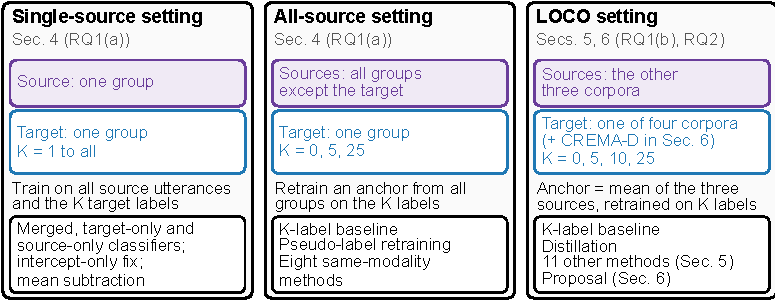
\includegraphics[width=\textwidth]{figures/fig_v2_settings_en.pdf}
\caption{The three settings. The single-source setting serves the analysis of S2, the all-source setting Sect.~4.2 of the main text and the LOCO setting Sects.~4.1 and 4.3--4.6. Groups: IEMOCAP improvised and scripted, MOSEI, MELD, AFEW, CREMA-D and RAVDESS}\label{fig:settings}
\end{figure}

\section{Details of the analysis}\label{sec:s2}
Figure~\ref{fig:twoerrors} illustrates the two parts of the error (Sect.~3.5 of the main text). Table~\ref{tab:methods} gives the K = 5 UARs of the 11 methods of Sect.~4.1; their references are self-training \cite{lee2013pseudolabel}, entropy minimisation \cite{grandvalet2004}, IM \cite{liang2020,boudiaf2020}, T3A \cite{iwasawa2021}, label propagation \cite{zhou2004,iscen2019}, CORAL \cite{sun2016coral}, DANN \cite{ganin2016dann}, MME \cite{saito2019mme} and xMUDA \cite{jaritz2020xmuda} (solved between unimodal classifiers). The next paragraphs give details of the main text and the single-source analysis moved from it.

\textbf{Formulas of the two parts of the error (Sect.~3.5 of the main text).} We quantify the two parts as follows. For the score $s_k(x)=w_k^\top x+b_k$ of emotion $k$, the decision between emotions $k$ and $l$ is the sign of $z_{kl}=(w_k-w_l)^\top x+(b_k-b_l)$. With mean $\hat\mu_k$ and variance $v_k$ of $z_{kl}$ over target test utterances of emotion $k$ (likewise for $l$) and $\sigma=\sqrt{(v_k+v_l)/2}$, we define
\begin{equation}
d_{kl}=\frac{\hat\mu_k-\hat\mu_l}{\sigma},\qquad o_{kl}=-\frac{\hat\mu_k+\hat\mu_l}{2\sigma},
\end{equation}
the separation of the two emotions on the decision axis and the offset of the boundary ($z_{kl}=0$) from the midpoint of their means. If $z_{kl}$ of both emotions is normal with equal variance, the pairwise accuracy is $A(d,o)=\tfrac12[\Phi(d/2-o)+\Phi(d/2+o)]$. With the separation $D^{*}$ along the linear discriminant direction of the labelled target utterances (Ledoit--Wolf shrinkage \cite{ledoit2004}), the pairwise loss splits as
\begin{equation}
A(D^{*},0)-A(d,o)=\underbrace{[A(D^{*},0)-A(d,0)]}_{\text{direction loss}}+\underbrace{[A(d,0)-A(d,o)]}_{\text{intercept loss}}.
\end{equation}
Changing only the intercepts shifts $z_{kl}$ equally for all utterances and moves only $o$; a shift $x\to x+\delta$ common to all emotions also moves only $o$, so subtracting each corpus's feature mean does not change the direction loss. $D^{*}$ is used only for evaluation and is not the largest separation over linear directions.

\textbf{Single-source analysis: one source corpus and the K labels mainly corrected prediction bias.} In the single-source setting, for each ordered pair of groups of Table~1 of the main text (target, source), all utterances of one source group and K = 5 target labels per emotion are trained together (merged classifier); classifiers trained on the source only and on the K target labels only (K = 1, 5, 10) are also built. The test set is one of five speaker folds of the target, and repetitions 0--9 change the folds and the test fold. The classifier weights carry an L2 penalty with inverse strength $C$ and the intercepts are unpenalised; $C\in\{0.01,0.1,1,10\}$ is chosen by speaker-split three-fold cross-validation (the merged classifier uses the $C$ of the source-only classifier of the same repetition). Audio features were also built from the last layer of HuBERT-large \cite{hsu2021} (Audio (HuBERT)). AFEW text features were made after these computations and are not used here. The comparisons are as follows (codes in Table~S9).
\begin{itemize}
\item \textbf{(A2) $-$ (A0):} the gain of adding the K labels to the source-only classifier (hereafter the merged gain).
\item \textbf{(A3) $-$ (A0) and (A4) $-$ (A0):} neither the intercept-only fix nor mean subtraction changes the direction loss (formulas above); the share of the merged gain that they obtain measures how much correcting prediction bias alone obtains.
\item \textbf{(A5) $-$ (A4):} whether correcting intercepts on the K labels adds to mean subtraction.
\item \textbf{The ratio $d_T(K)/D^{*}$ of (A1)} (K = 1, 5, 10): how close the weight direction comes to that of $D^{*}$ when only the K labels are used (remaining error).
\end{itemize}
Table~\ref{tab:s-single} shows these differences by feature set. For audio and visual features, the intercept-only fix (A3) and mean subtraction (A4) obtained most of the merged gain. The summed (A3) gain was 0.78--0.91 times the summed merged gain. Label-free (A4) gained 4.69\pt\ [3.81, 5.57] for audio (WavLM) against the merged 5.26\pt, and 2.40\pt\ for visual against 2.47\pt. The interval of (A5) $-$ (A4) was not above zero for any of the eight feature sets (two audio, visual, text and four concatenations).

For (A1), which uses no source, $d_T/D^{*}$ (median over targets of the ratio averaged over six emotion pairs) was 0.23, 0.47 and 0.62 for audio (WavLM) at K = 1, 5 and 10, and 0.11, 0.32 and 0.42 for text. Visual reached 1.01 at K = 10 (the ratio can exceed 1 because $D^{*}$ is not the largest linear separation).

\begin{table}[h]
\caption{Single-source setting (K = 5): UAR differences in points on test utterances; values are pair means (each pair averaged over repetitions 0--9); ``Ratio'' is $\sum$((A3) $-$ (A0)) $/ \sum$((A2) $-$ (A0)) over pairs; the last column gives 95\% intervals}\label{tab:s-single}
\footnotesize
\begin{tabular}{@{}lrrrl@{}}
\toprule
Features & (A2) $-$ (A0) & (A4) $-$ (A0) & Ratio & (A5) $-$ (A4) \\
\midrule
Audio (WavLM) & +5.26 & +4.69 & 0.91 & +0.38 [$-$0.12, +0.88] \\
Audio (HuBERT) & +4.73 & +4.18 & 0.90 & +0.18 [$-$0.42, +0.77] \\
Visual & +2.47 & +2.40 & 0.78 & $-$0.39 [$-$0.78, +0.02] \\
\botrule
\end{tabular}
\end{table}

This analysis has two limitations. First, the answer-bias result comes from the single-source setting, with target means over all utterances including test utterances. In the LOCO setting, an intercept-only fix on the K labels was below the baseline in point estimates in 18 of 32 conditions, so which error the K labels correct there is unknown. Second, the direction loss of visual features failed the pre-set fit criterion (see the paragraph on the fit of the approximation below), so the visual $d_T/D^{*}$ should be read as values that include errors of the same size as the approximation. Measuring the direction loss of an intercept-only fix in the LOCO setting is the next step.

\textbf{Gains of distillation for visual, text and AVT classifiers (Sect.~4.1 of the main text).} Table~\ref{tab:s-gain} adds the visual, text and AVT classifiers to the audio rows of Table~2 of the main text.

\begin{table}[h]
\caption{Classifier retrained by distillation $-$ baseline (UAR points on test utterances) with 95\% intervals without correction; mean of 50 repetitions (5 for K = 0). IEMOCAP: improvised part}\label{tab:s-gain}
\footnotesize\setlength{\tabcolsep}{3.4pt}
\begin{tabular}{@{}lllll@{}}
\toprule
Corpus & K = 0 & K = 5 & K = 10 & K = 25 \\
\midrule
\multicolumn{5}{@{}l}{\textit{Visual}} \\
AFEW & +2.48 [$-$1.34, +6.31] & +0.09 [$-$2.99, +3.17] & +0.18 [$-$1.90, +2.26] & $-$0.18 [$-$1.40, +1.04] \\
IEMOCAP & $-$2.08 [$-$5.19, +1.03] & $-$0.84 [$-$4.75, +3.06] & +0.91 [$-$4.76, +6.58] & $-$0.74 [$-$6.30, +4.82] \\
MOSEI & $-$0.91 [$-$2.35, +0.54] & +0.21 [$-$1.14, +1.56] & +1.56 [+0.16, +2.95] & +2.57 [+1.17, +3.98] \\
MELD & +0.67 [$-$2.76, +4.10] & +0.85 [$-$0.91, +2.61] & +0.71 [$-$0.50, +1.93] & +1.11 [$-$0.18, +2.40] \\
\multicolumn{5}{@{}l}{\textit{Text}} \\
AFEW & +1.56 [$-$2.33, +5.46] & +1.65 [$-$1.50, +4.79] & +1.83 [$-$0.92, +4.58] & +0.75 [$-$2.07, +3.56] \\
IEMOCAP & +7.52 [+4.75, +10.29] & +7.34 [+4.37, +10.31] & +6.87 [+3.06, +10.67] & +5.01 [+2.44, +7.57] \\
MOSEI & $-$0.69 [$-$1.72, +0.35] & $-$0.02 [$-$0.89, +0.84] & +0.79 [$-$0.02, +1.60] & +0.03 [$-$0.69, +0.74] \\
MELD & +0.18 [$-$2.56, +2.92] & $-$1.18 [$-$4.44, +2.08] & $-$1.28 [$-$3.15, +0.59] & $-$0.94 [$-$2.84, +0.95] \\
\multicolumn{5}{@{}l}{\textit{AVT}} \\
AFEW & +1.69 [$-$1.91, +5.30] & +1.03 [$-$0.65, +2.72] & +1.10 [$-$0.44, +2.65] & +0.62 [$-$0.33, +1.57] \\
IEMOCAP & +1.65 [$-$2.86, +6.16] & +0.16 [$-$4.53, +4.85] & +0.24 [$-$3.62, +4.09] & $-$0.83 [$-$5.12, +3.46] \\
MOSEI & $-$0.32 [$-$1.17, +0.54] & $-$0.35 [$-$0.90, +0.19] & +0.17 [$-$0.37, +0.70] & +0.74 [+0.18, +1.30] \\
MELD & +3.36 [+0.90, +5.81] & +2.53 [+1.65, +3.42] & +1.87 [+0.94, +2.80] & +1.41 [+0.63, +2.19] \\
\botrule
\end{tabular}
\end{table}


\textbf{Fit of the approximation (Sect.~3.5).} When the equal-variance Gaussian approximation was checked on source-only classifiers of the single-source setting, the median approximation error was 0.41--1.27 times the median intercept loss, failing the pre-set criterion (below 1/3), so prediction bias is measured by UAR differences rather than by the approximation (single-source analysis above). For the direction loss the ratio was 0.05--0.13, meeting the criterion except for visual features (0.47).

\textbf{Intervals and verdict rules of the single-source and all-source settings (Sect.~3.5).} Single-source intervals were percentile intervals of a two-stage bootstrap over speakers (clusters for MOSEI) and repetitions; for targets with fewer than 20 effective speakers, the union with a speaker-jackknife $t$ interval was used. In the all-source setting, hyperparameters were chosen with each source group as a provisional target, and intervals were two-stage bootstrap percentile intervals over speakers and repetitions, with the same resamples applied to a method and the baseline. By pre-set rules, a method \emph{reduced} the direction loss if the 95\% interval of (baseline $-$ method) was above zero and the point estimate at least $\delta$, \emph{increased} it if below zero and at most $-\delta$, was at the \emph{same level} if the interval lay within $\pm\delta$, and was \emph{undetermined} otherwise; $\delta$ (0.82--1.11\pt\ for the 81 conditions, 0.89--1.10\pt\ for the 210) was set from provisional-target outputs only.

\textbf{Excluded variants and exceptions among the other pseudo-label providers (Sects.~3.4 and 4.3).} AVT retrained on its own predictions and duplicates of other providers were excluded from the 360 variants per K. One excluded variant (MOSEI, AVT, K = 25), whose advantage is zero by construction because the provider makes the same predictions as the baseline, had a gain interval above zero (+0.30 [+0.07, +0.54]). Of the 36 variants with a positive advantage whose gain interval was below zero (16 at K = 5 and 20 at K = 25), 17 were for the text classifier on MOSEI and 8 for the visual classifier on MELD, and 28 used providers without the retrained classifier's own modality.

\textbf{Audio classifiers retrained without labels (Sect.~4.1).} The UARs of the audio classifier retrained on pseudo-labels alone (K = 0) and of the baseline with 5 and 10 labels per emotion were 53.4, 50.1 and 51.1 on AFEW, 69.2, 67.1 and 68.3 on IEMOCAP, 36.5, 34.9 and 35.1 on MOSEI and 45.2, 41.5 and 41.8 on MELD (no intervals computed).

\begin{figure}[h]
\centering
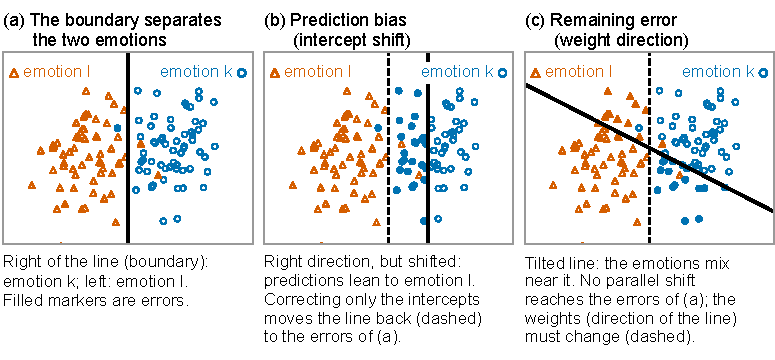
\includegraphics[width=\textwidth]{figures/fig_two_errors_v4_en.pdf}
\caption{Two parts of the error of a linear classifier, drawn in a two-dimensional feature space. (a) The boundary separates the two emotions. (b) Prediction bias: the direction is right but the boundary is shifted, biasing predictions towards one emotion; correcting only the intercept returns to (a). (c) Remaining error: the boundary is tilted, and no parallel shift brings the errors down to those of (a). The points are illustrative, not experimental data}\label{fig:twoerrors}
\end{figure}

\begin{table}[h]
\caption{LOCO setting, K = 5: UAR (points, test utterances; mean of 50 repetitions, 15 for the gradient-based DANN, MME and xMUDA-style methods). Numbers are those of Table~S9. *: interval of (C1) $-$ method above zero; $\dagger$: below zero (the method is higher). ``Own predictions'': the classifier's own (C0) probabilities as pseudo-labels. IEMOCAP: improvised part}\label{tab:methods}
\footnotesize\setlength{\tabcolsep}{4pt}
\begin{tabular}{@{}lllllllll@{}}
\toprule
 & \multicolumn{4}{c}{Audio} & \multicolumn{4}{c}{AVT} \\
Method & AFEW & IEMO. & MOSEI & MELD & AFEW & IEMO. & MOSEI & MELD \\
\midrule
(C1) Distillation (ref.) & 54.2 & 69.5 & 38.1 & 44.6 & 70.8 & 72.7 & 41.1 & 50.1 \\
(C0) K-label baseline (ref.) & 50.1 & 67.1 & 34.9 & 41.5 & 69.7 & 72.6 & 41.5 & 47.6 \\
(C2) Self-training & 50.1* & 67.1 & 32.0* & 40.7* & 72.1 & 71.3 & 40.4* & 46.1* \\
(C3) Entropy minimisation & 31.8* & 38.4* & 25.0* & 26.9* & 71.3 & 62.1* & 28.3* & 36.9* \\
(C4) IM & 50.6* & 66.8* & 34.6* & 40.5* & 70.4 & 70.6* & 39.4* & 39.6* \\
(C5) T3A & 44.3* & 57.1* & 30.7* & 34.0* & 72.0 & 65.5* & 37.4* & 41.7* \\
(C6) Label propagation & 45.3* & 58.6* & 32.3* & 31.0* & 59.8* & 61.0* & 34.5* & 33.6* \\
(C7) Own predictions & 50.6* & 66.8 & 35.0* & 41.9* & 69.9 & 71.6 & 41.6 & 47.9* \\
(C8) S+T & 50.2* & 62.1* & 35.5* & 41.1* & 64.5* & 70.2 & 41.1 & 51.8 \\
(C9) CORAL & 49.3* & 64.4* & 35.2* & 41.0* & 68.9 & 70.7 & 42.1$\dagger$ & 46.3* \\
(C10) DANN & 46.5* & 64.6* & 34.5* & 39.3* & 69.7 & 71.6 & 40.5 & 47.1* \\
(C11) MME & 46.5* & 63.4* & 30.8* & 33.3* & 70.4 & 63.0* & 34.8* & 31.2* \\
(C12) xMUDA-style & 48.8* & 68.9 & 35.7* & 37.5* & --- & --- & --- & --- \\
\botrule
\end{tabular}
\end{table}

\section{Can audio features predict the text classifier's decisions?}\label{sec:s3}
As one candidate reason for the audio gains in Sect.~4.1 of the main text (discussed in Sect.~5), we examined whether audio features can predict the text classifier's decisions contained in the product.

\subsection{Setting}
We examined the explanation that speech carries both voice quality and the spoken words: the product contains the text classifier's decisions, so if audio features can predict those decisions, the audio classifier can learn that part from the pseudo-labels. The cross-modal predictability $D$ is measured as follows: the decisions $J$ of one modality's K-label baseline (e.g., text) are the target; a linear classifier on another modality's features (e.g., audio) predicts $J$ out of sample, and its UAR with $J$ as truth is $R$; the same is done after permuting $J$ within strata of true emotion and speaker cluster (and gender for IEMOCAP and AFEW), giving $R'$; and $D=R-R'$ is the agreement not explained by emotion and speaker (Fig.~\ref{fig:dtoy}). The decision rule was fixed at K = 5 before computing, and AFEW, whose text is a transcript of its own audio, was excluded from the audio--text comparison. We also rebuilt the last-layer WavLM-large features of time-reversed speech of IEMOCAP (improvised), MOSEI and MELD and measured the same $D$ (predictions and rules fixed before computing; the question was set after seeing the non-reversed results). On reversed speech, Whisper large-v3 transcripts agreed with the original words only 0.005--0.012 above chance (0.79--0.80 for the original speech).



\begin{figure}[t]
\centering
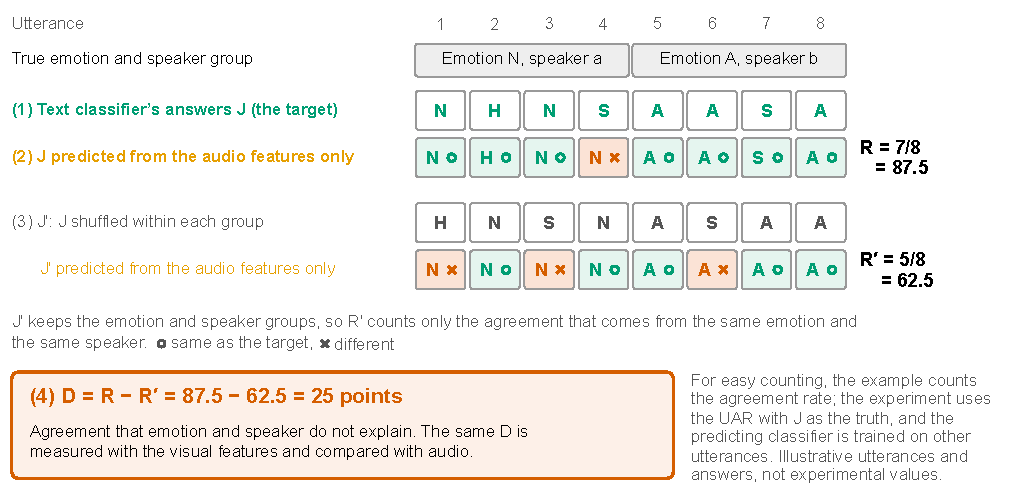
\includegraphics[width=\textwidth]{figures/fig_D_toy_en.pdf}
\caption{Measuring the predictability $D$ (illustrative example). The text classifier's decisions $J$ are predicted from audio features only ($R$), and so are $J'$, the decisions $J$ shuffled within groups of the same emotion and speaker ($R'$); $D=R-R'$. The example counts the agreement rate; the experiment uses the UAR with $J$ as truth. Utterances and decisions are illustrative}\label{fig:dtoy}
\end{figure}

\subsection{Results: audio features predicted the text classifier's decisions better than visual features}
On the three corpora other than AFEW, the predictability $D$ of the text classifier's decisions was 19.3 (IEMOCAP), 10.5 (MOSEI) and 17.7 (MELD) points with audio features and 2.0, 0.3 and 3.8 with visual features; the differences (+17.3, +10.2, +13.9) all had intervals above zero. Audio features did not meet the pre-set rule at K = 5 for predicting the visual classifier's decisions better than text features. $D$ may also include agreement from arousal, speaker attributes, utterance duration and recording conditions. Reversing the speech lowered $D$ to 10.5, 3.1 and 10.5 (differences 8.8 [3.0, 14.7], 7.5 [6.3, 8.6] and 7.2 [4.7, 9.8]) (Fig.~\ref{fig:reverse}), but reversed audio still exceeded visual features (by 8.5 [3.8, 13.1], 2.7 [1.3, 4.1] and 6.7 [3.8, 9.6]). Audio's prediction of the text classifier's decisions was therefore not explained by intelligible words alone; the remainder may come from the average spectrum, the pitch distribution, utterance duration, intensity differences within an emotion label or word information left in WavLM features, which this experiment cannot separate.

\begin{figure}[t]
\centering
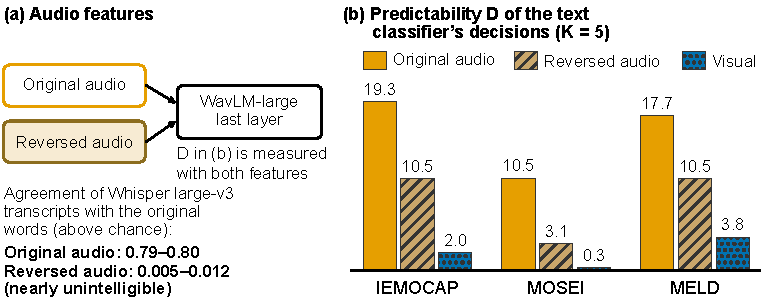
\includegraphics[width=\textwidth]{figures/fig_reverse_en.pdf}
\caption{Predictability $D$ of the text classifier's decisions at K = 5 (UAR points) by original audio, time-reversed audio (words nearly unintelligible) and visual features. The visual value is the reversed-audio $D$ minus the measured difference (reversed audio $-$ visual). AFEW is excluded because its text is a transcript of its own audio}\label{fig:reverse}
\end{figure}


\textbf{Limitation.} Reversed speech was checked with Whisper transcripts, not with human listeners. Reversal also inverts time-directional cues such as intonation contours and produces speech unlike the data WavLM was trained on, so the drop in $D$ should not be attributed to intelligible words alone; measuring $D$ with another manipulation that makes words unintelligible is the next step.

\section{Details of the distillation loss}\label{sec:s4}
The loss of distillation in Sect.~3.4 of the main text (form (a), without temperature) was fixed before the evaluation run. The loss hyperparameters $\rho\in\{1/16,1/4,1,4\}$ and $a\in\{1,4,16\}$ and the exponents of each modality in the product (63 combinations of $\{0,0.5,1,2\}^3$ excluding all zeros) were set to the point with the highest mean UAR over provisional targets (Sect.~3.7 of the main text); when several points were within two standard errors of the best, the one closest to the untuned values ($\rho=1$, $a=1$, exponents (1, 1, 1)) was chosen. For comparison, five other loss forms that take the pseudo-labels were trained in the same way, and for each target, classifier and K the form with the highest provisional-target UAR was compared with form (a): a temperature loss (form (b)) \cite{hinton2015distilling} with $\tau=2$ from Albanie et al.\ \cite{albanie2018}, pseudo-labels on agreeing utterances only \cite{shi2024audioguided}, mixing with the classifier's own predictions \cite{zhang2021combining}, soft co-training (our variant of the idea of \cite{blum1998}) and co-regularisation \cite{sindhwani2005coreg}; each adapts the loss of the original paper to take the pseudo-labels as targets and is not identical to the original method. Replacing form (a) by the form selected on provisional targets (form (b) in all 16 audio conditions with K = 0, 5, 10, 25) changed audio UAR by $-$0.79 to +0.87\pt, and the selected hyperparameters gave the same classifier as the untuned values in all 16 audio conditions. These results suggest that the audio gains did not come from the choice of loss form or of hyperparameters.

\section{Method details and comparators}\label{sec:s5}
Figure~\ref{fig:decomp} illustrates the weight table of Sect.~3.6 of the main text, Fig.~\ref{fig:episode} the hyperparameter selection of Sect.~3.6, and Table~\ref{tab:comparators} the content and references of the comparators of Sect.~4.4 and Sect.~\ref{sec:s6}.

\textbf{Where to measure strengths and profiles (Sect.~3.6).} In the provisional-target computations used to design the method, two classifier-by-emotion reliability tables were built, one measured on the sources and one on all candidate labels of the provisional target (ranges below are minima and maxima over four corpora $\times$ K = 5, 10, 25). The correlation between the three classifier strengths in the two tables was $-$0.954 to +0.403, and the strongest modality agreed between the two in 0--0.467 of repetitions (0.433--1.000 for strengths measured on the K labels, which agreed less often than the source-measured strengths only on MOSEI at K = 25, 0.433 vs 0.467). The classifier-by-emotion component left after fitting classifier and emotion effects and Tukey's one-degree-of-freedom non-additivity term \cite{tukey1949} correlated 0.463--0.780 between the two tables.

\textbf{Agreement of the classifier with the highest K-label strength in the evaluation (Sect.~4.5).} Counted after the evaluation over its 50 repetitions, the classifier with the highest K-label strength was the one with the highest strength on all candidate labels (visual on AFEW, audio on IEMOCAP, text on MELD) in 0.94, 0.96 and 1.00 of repetitions on AFEW, 0.86, 0.92 and 1.00 on IEMOCAP, and 0.70, 0.76 and 0.88 on MELD (K = 5, 10, 25). On MOSEI this fraction was 0.30, 0.36 and 0.38.

\begin{figure}[h]
\centering
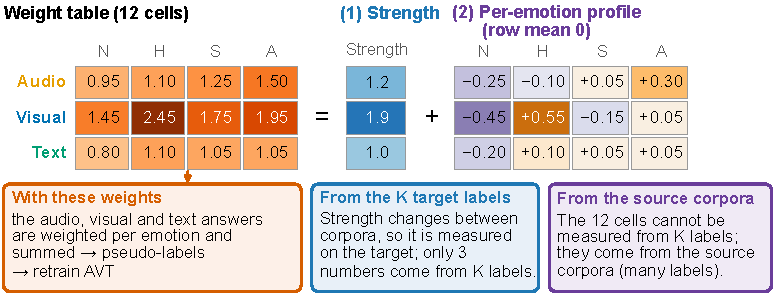
\includegraphics[width=\textwidth]{figures/fig_prop_decomp_en.pdf}
\caption{The 12-cell classifier-by-emotion weight table split into (1) one strength per classifier, measured on the K target labels (three numbers), and (2) per-emotion profiles, measured on the source corpora (each row sums to zero). Numbers are illustrative}\label{fig:decomp}
\end{figure}

\begin{figure}[h]
\centering
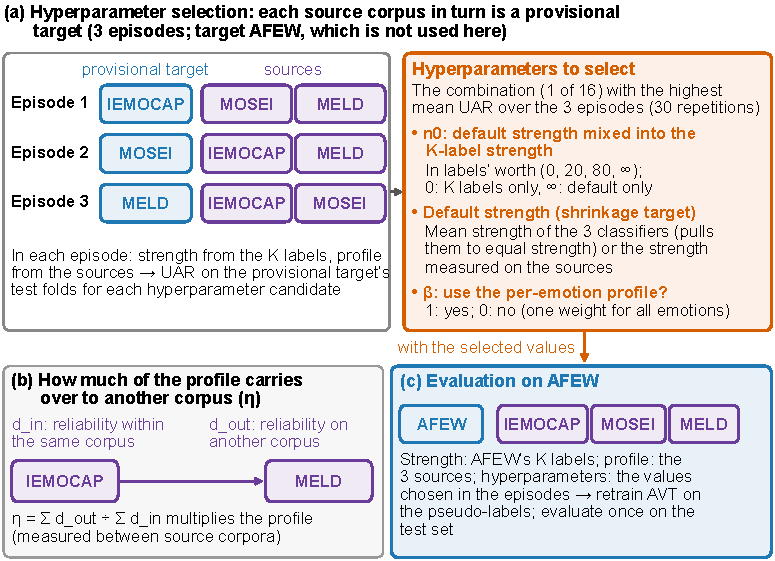
\includegraphics[width=\textwidth]{figures/fig_prop_episode_en.pdf}
\caption{Hyperparameter selection (target AFEW). In three episodes, each source corpus serves as a provisional target; strengths are measured on its K labels and profiles on the other two sources, and the hyperparameter setting with the highest mean UAR on the provisional targets' test folds is chosen. The carry-over $\eta$ of the profiles is measured between sources. AFEW is then evaluated once with the selected values}\label{fig:episode}
\end{figure}

\begin{table}[h]
\caption{Comparators. Numbers are those of Table~S9; rows without numbers are the comparators of Sect.~\ref{sec:s6}. ``From K'' is the number of quantities fitted or selected on the K target labels (the proposal: three strengths)}\label{tab:comparators}
\footnotesize\setlength{\tabcolsep}{4pt}
\begin{tabular}{@{}lp{2.8cm}p{4.0cm}p{2.5cm}l@{}}
\toprule
No. & Comparison & Content & Reference & From K \\
\midrule
(D0) & Product & Multiply the three probabilities with equal weights & Product rule \cite{kittler1998} & 0 \\
(D1) & Mean of probabilities & Average the three probabilities & Sum rule \cite{kittler1998} & 0 \\
-- & Strength-only weights & Sum scores with weights proportional to the K-label strengths, common to emotions & Classifier weights \cite{kuncheva2014} & 3 \\
-- & Full table from K & All 12 reliabilities measured on the K labels, combined as the proposal & Same number of per-class parameters as a recall combiner \cite{kuncheva2014} & 12 \\
(D2) & Temperature calibration & Per-classifier inverse temperatures fitted to the K-label log-likelihood, then multiplied & Temperature scaling \cite{guo2017calibration} & 3 \\
-- & Weight-table search & Among 1,000 random tables and the equal table, the one with the highest K-label UAR & Random search as in Kaya et al.\ \cite{kaya2017} & 1 of 1,001 \\
(D3) & Strongest single classifier & Predictions of the product component with the highest K-label strength & Added in this study & 1 of 3 \\
(E0) & Baseline AVT & Retrain on the K labels without pseudo-labels & Sect.~3.1 & --- \\
(E1) & Distillation (product) & Retrain AVT on the product's pseudo-labels & Sect.~3.4 & --- \\
\botrule
\end{tabular}
\end{table}

\textbf{Details of the comparison with the strongest single classifier (Sect.~4.4 of the main text).} This comparison was built after the evaluation run from saved outputs (outside the evaluation protocol), with the same label-free intercept shift as the proposal. On AFEW at K = 5, this method (68.65) was lower than the visual classifier alone (70.70) because it selected a non-visual classifier in 3 of 50 repetitions and its intercepts were shifted (69.25 before the shift); the shift lowered it on AFEW by 0.44--0.65\pt, and without the shift for either method proposal $-$ strongest single was +1.86 to +6.11\pt\ in all 12 conditions (intervals above zero in eight). By contrast, per-emotion recall of the proposal was lower than that of this method in point estimates for Happy on AFEW ($-$6.42 to $-$4.39\pt), Neutral on MELD ($-$4.32 to $-$2.74\pt) and Sad on IEMOCAP at K = 25 ($-$0.21\pt; no per-emotion intervals computed). Decomposing the difference, product $-$ strongest single (+2.04 to +5.02\pt; intervals above zero in 7 of 9) accounted for most of it on IEMOCAP, MOSEI and MELD, and proposal $-$ product on AFEW (product $-$ strongest single +0.57 to +0.67\pt).

\section{Further comparisons of the proposal}\label{sec:s6}
\subsection{Comparators fitted on the K labels}
Against the three comparators that fit weights on the K labels (Table~\ref{tab:s1}), the proposal's fused predictions differed by $-$1.16 to +0.73\pt\ from strength-only weights, with intervals above zero on MOSEI at all K and on IEMOCAP at K = 5, and was higher in point estimates in 9 of 12 conditions than all 12 reliabilities measured on the K labels and in 11 of 12 than selecting one of 1,001 tables.

\begin{table}[h]
\caption{UAR of the three comparators fitted on the K labels (points, test utterances, mean of 50 repetitions; not in Table~S10). Parentheses: proposal's fused predictions $-$ row with 95\% intervals without correction; * interval above zero, $\dagger$ below zero. Intervals of the weight-table search are conditional on the drawn tables. Strength-only weights gave the same UAR as the proposal without per-emotion profiles (Table~S10) in 8 of the 12 conditions on the four corpora and in all three on CREMA-D (Table~S8)}\label{tab:s1}
\footnotesize\setlength{\tabcolsep}{2pt}
\begin{tabular}{@{}llll@{}}
\toprule
Row & K = 5 & K = 10 & K = 25 \\
\midrule
\multicolumn{4}{@{}l}{\textbf{AFEW}} \\
Strength only & 72.51 ($-$1.16 [$-$2.6, +0.3]) & 73.94 (+0.45 [$-$0.1, +1.0]) & 76.55 (+0.03 [$-$0.5, +0.6]) \\
Full table (K) & 72.55 ($-$1.19 [$-$2.8, +0.4]) & 74.34 (+0.05 [$-$0.6, +0.7]) & 76.84 ($-$0.26 [$-$0.8, +0.3]) \\
Table search & 71.50 ($-$0.14 [$-$2.4, +2.1]) & 73.80 (+0.59 [$-$1.2, +2.3]) & 76.55 (+0.03 [$-$1.9, +1.9]) \\
\multicolumn{4}{@{}l}{\textbf{IEMOCAP (improvised)}} \\
Strength only & 72.32 (+0.24 [+0.03, +0.5]*) & 73.57 (+0.23 [$-$0.05, +0.5]) & 74.83 (+0.20 [$-$0.1, +0.5]) \\
Full table (K) & 72.36 (+0.20 [$-$1.7, +2.1]) & 73.75 (+0.05 [$-$0.7, +0.8]) & 75.30 ($-$0.27 [$-$1.1, +0.5]) \\
Table search & 70.41 (+2.15 [+0.9, +3.4]*) & 71.30 (+2.50 [+1.7, +3.3]*) & 73.49 (+1.54 [+1.2, +1.9]*) \\
\multicolumn{4}{@{}l}{\textbf{MOSEI}} \\
Strength only & 40.43 (+0.73 [+0.5, +1.0]*) & 42.20 (+0.62 [+0.4, +0.9]*) & 43.96 (+0.51 [+0.3, +0.8]*) \\
Full table (K) & 40.62 (+0.54 [$-$0.01, +1.1]) & 42.31 (+0.51 [+0.1, +0.9]*) & 44.08 (+0.39 [+0.1, +0.7]*) \\
Table search & 40.06 (+1.10 [+0.6, +1.6]*) & 41.48 (+1.34 [+0.9, +1.8]*) & 42.80 (+1.66 [+1.2, +2.1]*) \\
\multicolumn{4}{@{}l}{\textbf{MELD}} \\
Strength only & 50.52 ($-$0.46 [$-$1.3, +0.3]) & 50.89 ($-$0.20 [$-$1.0, +0.6]) & 52.80 (+0.15 [$-$0.1, +0.4]) \\
Full table (K) & 49.37 (+0.68 [$-$0.2, +1.5]) & 50.39 (+0.29 [$-$0.4, +1.0]) & 52.53 (+0.42 [$-$0.02, +0.9]) \\
Table search & 49.47 (+0.59 [$-$0.5, +1.7]) & 49.67 (+1.01 [+0.1, +2.0]*) & 51.47 (+1.48 [+0.7, +2.3]*) \\
\botrule
\end{tabular}
\end{table}


\subsection{Four further combinations of the same predictions}
Table~\ref{tab:extra} compares the proposal's fused predictions with four further combinations of the predictions of the same product components, computed in the same evaluation run as Table~S10; the proposal and each combination use the label-free intercept shift of Sect.~3.6 of the main text. \emph{Exponents from other corpora} (selected separately from the untuned exponents of distillation and the product) multiplies the three probabilities raised to one exponent per modality (common to emotions), chosen on the provisional-target runs of Sect.~3.4 of the main text and normalised to mean 1; on AFEW the selected exponents were (1, 1, 1), so its decisions equal those of the product. \emph{Confidence-weighted mean} averages the three probabilities, each weighted per utterance by the classifier's maximum probability (a confidence-weighted late fusion used as a baseline by Tellamekala et al.\ \cite{tellamekala2024}; using the maximum probability as the confidence is our choice). \emph{Table re-reading} re-reads each classifier's probabilities with a diagonal confusion table measured on the K labels (off-diagonal entries $(1-\text{diagonal})/3$), shrunk halfway towards a table with the classifier's mean diagonal, and multiplies them; classifiers whose mean diagonal is at most 0.25 are not used. \emph{Modality weights from K} fits three modality weights (common to emotions) jointly to the log-likelihood of the combined prediction on the K labels (a weighted log-linear pool \cite{heskes1997}). Of the 48 conditions, the difference was positive in 39, with intervals above zero in 25 and below zero in none.

\begin{table}[h]
\caption{Proposal's fused predictions $-$ further combinations (UAR points, test utterances, mean of 50 repetitions) with 95\% intervals without correction. * interval above zero (proposal higher); $\dagger$ below zero. IEMOCAP: improvised part}\label{tab:extra}
\footnotesize\setlength{\tabcolsep}{3pt}
\begin{tabular}{@{}llll@{}}
\toprule
Corpus & K = 5 & K = 10 & K = 25 \\
\midrule
\multicolumn{4}{@{}l}{\textit{Exponents from other corpora}} \\
AFEW & +2.13 [+1.0, +3.3]* & +3.51 [+1.5, +5.5]* & +3.14 [+1.9, +4.4]* \\
IEMOCAP & +2.52 [+0.4, +4.6]* & +2.36 [+0.6, +4.1]* & +2.72 [+1.4, +4.0]* \\
MOSEI & +0.45 [$-$0.02, +0.9] & +0.49 [+0.04, +0.9]* & +0.57 [+0.1, +1.0]* \\
MELD & +2.10 [+0.5, +3.7]* & +2.42 [+1.5, +3.3]* & +2.94 [+1.7, +4.2]* \\
\multicolumn{4}{@{}l}{\textit{Confidence-weighted mean}} \\
AFEW & +2.07 [+0.7, +3.5]* & +3.23 [+1.7, +4.8]* & +3.31 [+1.8, +4.8]* \\
IEMOCAP & +0.07 [$-$1.5, +1.6] & +0.11 [$-$2.2, +2.4] & +0.14 [$-$2.1, +2.3] \\
MOSEI & +0.24 [$-$0.2, +0.6] & +0.33 [$-$0.1, +0.7] & +0.71 [+0.4, +1.1]* \\
MELD & +0.01 [$-$1.3, +1.3] & +0.45 [$-$0.4, +1.3] & +0.93 [+0.2, +1.7]* \\
\multicolumn{4}{@{}l}{\textit{Table re-reading}} \\
AFEW & $-$0.63 [$-$1.9, +0.6] & +0.71 [$-$0.2, +1.6] & +0.29 [$-$0.8, +1.4] \\
IEMOCAP & $-$0.39 [$-$2.6, +1.8] & $-$0.48 [$-$2.3, +1.4] & $-$0.82 [$-$3.1, +1.5] \\
MOSEI & +1.98 [+1.1, +2.9]* & +1.18 [+0.6, +1.7]* & +1.08 [+0.6, +1.6]* \\
MELD & +1.10 [$-$0.2, +2.3] & +0.39 [$-$0.7, +1.5] & +0.21 [$-$0.5, +1.0] \\
\multicolumn{4}{@{}l}{\textit{Modality weights from K}} \\
AFEW & $-$3.54 [$-$8.0, +0.9] & $-$1.57 [$-$4.8, +1.6] & $-$1.50 [$-$3.8, +0.8] \\
IEMOCAP & +2.30 [+0.6, +4.0]* & +1.38 [+0.4, +2.3]* & +0.90 [+0.5, +1.3]* \\
MOSEI & +2.30 [+1.6, +3.0]* & +1.61 [+1.0, +2.2]* & +0.90 [+0.4, +1.4]* \\
MELD & +0.57 [$-$0.6, +1.8] & $-$0.15 [$-$1.4, +1.1] & $-$0.08 [$-$0.7, +0.6] \\
\botrule
\end{tabular}
\end{table}



\section{CREMA-D}\label{sec:s7}
CREMA-D was added to the evaluation after its values had been seen in six-corpus provisional-target computations (Sect.~3.7 of the main text). Proposal $-$ product of the fused predictions and AV retrained on the proposal's pseudo-labels $-$ AV retrained on the product's pseudo-labels were +0.31 to +0.63\pt\ with all six intervals excluding zero, and the difference from the proposal without per-emotion profiles had intervals above zero at all K.

\begin{table}[h]
\caption{CREMA-D (audio and visual): UAR (points, test utterances, mean of 50 repetitions; not in Table~S10). Rows and marks as in Table~S10, with AV in place of AVT for the retrained classifiers; rows without counterparts in Table~S10 are the comparators of Sect.~\ref{sec:s6}. The strongest single classifier was not computed for CREMA-D}\label{tab:s3}
\footnotesize\setlength{\tabcolsep}{1pt}
\begin{tabular}{@{}p{2.2cm}lll@{}}
\toprule
Row & K = 5 & K = 10 & K = 25 \\
\midrule
Proposal (fused) & 85.48 & 86.17 & 87.70 \\
Product & 85.01 (+0.47 [+0.2, +0.8]*) & 85.54 (+0.63 [+0.3, +0.9]*) & 87.13 (+0.57 [+0.3, +0.9]*) \\
Probability mean & 84.70 (+0.78 [+0.4, +1.2]*) & 85.23 (+0.94 [+0.5, +1.4]*) & 86.92 (+0.77 [+0.3, +1.2]*) \\
Strength only & 85.26 (+0.23 [+0.1, +0.4]*) & 85.89 (+0.27 [+0.1, +0.4]*) & 87.46 (+0.23 [+0.05, +0.4]*) \\
Full table (K) & 85.19 (+0.29 [$-$0.01, +0.6]) & 86.05 (+0.11 [$-$0.1, +0.4]) & 87.71 ($-$0.01 [$-$0.2, +0.2]) \\
Temperature calibration & 85.26 (+0.22 [$-$0.1, +0.5]) & 86.04 (+0.12 [$-$0.1, +0.4]) & 87.55 (+0.14 [$-$0.1, +0.4]) \\
Table search & 84.24 (+1.24 [+0.5, +2.0]*) & 85.46 (+0.71 [+0.1, +1.3]*) & 86.75 (+0.94 [+0.5, +1.4]*) \\
Without profiles & +0.23 [+0.1, +0.4]* & +0.27 [+0.1, +0.4]* & +0.23 [+0.05, +0.4]* \\
Without strength differences & +0.19 [$-$0.1, +0.4] & +0.28 [+0.04, +0.5]* & +0.36 [+0.1, +0.6]* \\
AV, proposal pseudo-labels & 85.64 & 86.53 & 87.74 \\
Baseline AV & 82.34 (+3.30 [+2.6, +4.0]*) & 83.35 (+3.18 [+2.5, +3.8]*) & 85.34 (+2.40 [+1.9, +2.9]*) \\
AV, product pseudo-labels & 85.32 (+0.31 [+0.1, +0.6]*) & 86.01 (+0.52 [+0.3, +0.8]*) & 87.35 (+0.39 [+0.1, +0.7]*) \\

\botrule
\end{tabular}
\end{table}

\section{Codes of the compared conditions}\label{sec:s8}
Tables~S4 and S5 call the compared conditions by the codes of Table~\ref{tab:s-codes}; the main text calls them by name.

\begin{table}[!htbp]
\caption{Codes of the compared conditions, used in Tables~S4 and S5; the main text calls the conditions by name. \checkmark: the condition uses the information source; --: it does not}\label{tab:s-codes}
\footnotesize\setlength{\tabcolsep}{3pt}
\begin{tabular}{@{}l p{6.3cm} cccc@{}}
\toprule
No. & Condition & Source & K & Unl. & Other \\
\midrule
\multicolumn{6}{@{}p{12.6cm}@{}}{\textbf{A: single-source setting} (ordered pairs of the 7 groups, K = 5; (A1) K = 1, 5, 10)} \\
(A0) & Source-only classifier & \checkmark & -- & -- & -- \\
(A1) & Target-only classifier & -- & \checkmark & -- & -- \\
(A2) & Merged classifier (all source utterances and the K labels trained together) & \checkmark & \checkmark & -- & -- \\
(A3) & Intercept-only fix (weights of (A0) fixed; only intercepts learned on the K labels) & \checkmark & \checkmark & -- & -- \\
(A4) & Mean subtraction (the mean of all utterances is subtracted from source and target features before retraining) & \checkmark & -- & \checkmark$^{a}$ & -- \\
(A5) & Intercepts corrected on the K labels after mean subtraction & \checkmark & \checkmark & \checkmark$^{a}$ & -- \\
\multicolumn{6}{@{}p{12.6cm}@{}}{\textbf{B: all-source setting} (K = 0, 5, 25; (B2)--(B9) K = 0, 5)} \\
(B0) & K-label baseline (anchor retrained on the K labels) & \checkmark & \checkmark & -- & -- \\
(B1) & Distillation (retrained on pseudo-labels from classifiers including other modalities) & \checkmark & \checkmark & \checkmark & \checkmark \\
(B2)--(B9) & Eight methods that use same-modality unlabelled utterances$^{b}$ & \checkmark & \checkmark & \checkmark & -- \\
\multicolumn{6}{@{}p{12.6cm}@{}}{\textbf{C: LOCO setting} (AFEW, IEMOCAP, MOSEI, MELD; K = 0, 5, 10, 25; (C2)--(C12) K = 5, 10, 25; (C13) K = 5, 25)} \\
(C0) & K-label baseline (audio, visual, text, AVT) & \checkmark & \checkmark & -- & -- \\
(C1) & Distillation (retrained on the product pseudo-labels) & \checkmark & \checkmark & \checkmark & \checkmark \\
(C2)--(C11) & Ten methods that use no information from other modalities$^{c}$ & \checkmark & \checkmark & \checkmark$^{c}$ & -- \\
(C12) & xMUDA-style mutual mimicry between unimodal classifiers (no pseudo-labels including other modalities)$^{c}$ & \checkmark & \checkmark & \checkmark & \checkmark \\
(C13) & Retraining with other pseudo-label providers (360 variants per K) & \checkmark & \checkmark & \checkmark & \checkmark\ or --$^{d}$ \\
\multicolumn{6}{@{}p{12.6cm}@{}}{\textbf{D: LOCO setting, fused predictions} (K = 5, 10, 25; CREMA-D in the SI)} \\
(D0) & Product (of the probabilities of the three classifiers that make the pseudo-labels of (C1)) & \checkmark & \checkmark & \checkmark & \checkmark \\
(D1) & Probability mean (sum rule) & \checkmark & \checkmark & \checkmark & \checkmark \\
(D2) & Per-classifier temperature calibration (fitted by log-likelihood on the K labels) & \checkmark & \checkmark & \checkmark & \checkmark \\
(D3) & Decisions of the single classifier strongest on the K labels & \checkmark & \checkmark & \checkmark & \checkmark \\
(D4) & Proposal (Sect.~3.6 of the main text) & \checkmark & \checkmark & \checkmark & \checkmark \\
(D5) & Proposal without per-emotion profiles & \checkmark & \checkmark & \checkmark & \checkmark \\
(D6) & Proposal without strength differences & \checkmark & \checkmark & \checkmark & \checkmark \\
\multicolumn{6}{@{}p{12.6cm}@{}}{\textbf{E: LOCO setting, retrained AVT} (K = 5, 10, 25)} \\
(E0) & K-label baseline AVT (the AVT of (C0)) & \checkmark & \checkmark & -- & -- \\
(E1) & AVT retrained on the product pseudo-labels (the AVT of (C1)) & \checkmark & \checkmark & \checkmark & \checkmark \\
(E2) & AVT retrained on the proposal's pseudo-labels & \checkmark & \checkmark & \checkmark & \checkmark \\
\botrule
\end{tabular}
\footnotetext{$^{a}$The target mean is taken over all target utterances including the test utterances; no labels are used. $^{b}$(B2) entropy minimisation, (B3) self-training, (B4) IM, (B5) T3A, (B6) label propagation, (B7) CORAL, (B8) DANN, (B9) MME. $^{c}$(C2) self-training, (C3) entropy minimisation, (C4) IM, (C5) T3A, (C6) label propagation, (C7) pseudo-labels from the retrained classifier's own (C0) probabilities, (C8) training on labelled source utterances and the K labels together (S+T), (C9) CORAL, (C10) DANN, (C11) MME, (C12) xMUDA-style. (C8)--(C11) also train on the source utterances themselves, and (C8) uses no unlabelled target utterances. (C2)--(C12) are the 11 methods that do not use pseudo-labels including other modalities; (C12) was computed only for the audio, visual and text classifiers. For group D, ``Other'' means that predictions of the three modalities are combined; the single classifier of (D3) was retrained on the probabilities of the AVT classifier (Sect.~3.4 of the main text). $^{d}$Depending on the provider, the pseudo-labels do or do not include predictions of other modalities (providers listed in Sect.~3.4 of the main text)}
\end{table}

\section{Full evaluation table of the proposal}\label{sec:s9}
Table~\ref{tab:s-full} gives the UARs and differences counted in Table~4 of the main text.

\begin{table}[!htbp]
\caption{UARs of the fused predictions and of retrained AVT (points, test utterances, mean of 50 repetitions). Parentheses: for the fused predictions, proposal $-$ row; for retrained AVT, AVT retrained on the proposal's pseudo-labels $-$ row; 95\% intervals without correction. Rows without the proposal's parts give only the difference. * interval above zero (proposal higher); $\dagger$ below zero (proposal lower). The strongest single classifier was added after the evaluation run (Sect.~3.7 of the main text)}\label{tab:s-full}
\footnotesize\setlength{\tabcolsep}{1pt}
\begin{tabular}{@{}p{2.2cm}lll@{}}
\toprule
Row & K = 5 & K = 10 & K = 25 \\
\midrule
\multicolumn{4}{@{}l}{\textbf{AFEW}} \\
Proposal (fused) & 71.36 & 74.39 & 76.58 \\
Product & 69.23 (+2.13 [+1.0, +3.3]*) & 70.88 (+3.51 [+1.5, +5.5]*) & 73.45 (+3.14 [+1.9, +4.4]*) \\
Probability mean & 69.22 (+2.14 [+1.0, +3.2]*) & 71.02 (+3.38 [+1.9, +4.9]*) & 72.85 (+3.73 [+2.5, +5.0]*) \\
Temperature calibration & 74.30 ($-$2.94 [$-$5.6, $-$0.3]$\dagger$) & 74.84 ($-$0.45 [$-$1.5, +0.6]) & 76.31 (+0.27 [$-$0.6, +1.1]) \\
Strongest single & 68.65 (+2.70 [$-$3.3, +8.7]) & 70.21 (+4.18 [$-$1.2, +9.6]) & 72.79 (+3.79 [$-$1.5, +9.1]) \\
Without profiles & +0.38 [+0.03, +0.7]* & +0.45 [$-$0.1, +1.0] & +0.36 [$-$0.2, +1.0] \\
Without strength differences & +1.74 [+0.4, +3.1]* & +3.20 [+1.1, +5.3]* & +2.57 [+1.4, +3.7]* \\
AVT, proposal pseudo-labels & 71.78 & 74.61 & 77.05 \\
Baseline AVT & 69.74 (+2.04 [+0.5, +3.6]*) & 71.56 (+3.05 [+1.8, +4.3]*) & 75.22 (+1.83 [+0.9, +2.8]*) \\
AVT, product pseudo-labels & 70.77 (+1.01 [+0.2, +1.8]*) & 72.66 (+1.95 [+0.5, +3.4]*) & 75.84 (+1.21 [+0.4, +2.0]*) \\
\midrule
\multicolumn{4}{@{}l}{\textbf{IEMOCAP (improvised)}} \\
Proposal (fused) & 72.56 & 73.80 & 75.03 \\
Product & 72.07 (+0.49 [$-$0.2, +1.2]) & 73.37 (+0.43 [$-$0.2, +1.1]) & 74.53 (+0.50 [+0.01, +1.0]*) \\
Probability mean & 73.03 ($-$0.46 [$-$2.8, +1.9]) & 74.25 ($-$0.46 [$-$3.1, +2.2]) & 75.52 ($-$0.49 [$-$3.2, +2.2]) \\
Temperature calibration & 71.69 (+0.87 [+0.5, +1.2]*) & 73.16 (+0.64 [$-$0.1, +1.4]) & 74.37 (+0.67 [$-$0.2, +1.6]) \\
Strongest single & 67.05 (+5.52 [+1.3, +9.8]*) & 68.42 (+5.38 [$-$0.5, +11.2]) & 71.51 (+3.52 [$-$3.6, +10.7]) \\
Without profiles & +0.24 [+0.03, +0.5]* & +0.23 [$-$0.05, +0.5] & +0.20 [$-$0.1, +0.5] \\
Without strength differences & +0.38 [$-$0.2, +1.0] & +0.06 [$-$0.6, +0.7] & +0.22 [$-$0.3, +0.7] \\
AVT, proposal pseudo-labels & 72.81 & 73.86 & 74.95 \\
Baseline AVT & 72.55 (+0.25 [$-$4.5, +5.0]) & 73.49 (+0.36 [$-$3.7, +4.4]) & 75.51 ($-$0.56 [$-$4.7, +3.6]) \\
AVT, product pseudo-labels & 72.71 (+0.10 [$-$0.6, +0.8]) & 73.73 (+0.13 [$-$0.3, +0.6]) & 74.68 (+0.27 [$-$0.1, +0.6]) \\
\midrule
\multicolumn{4}{@{}l}{\textbf{MOSEI}} \\
Proposal (fused) & 41.16 & 42.82 & 44.47 \\
Product & 40.97 (+0.19 [$-$0.2, +0.6]) & 42.53 (+0.29 [$-$0.03, +0.6]) & 44.07 (+0.40 [+0.1, +0.7]*) \\
Probability mean & 41.01 (+0.15 [$-$0.2, +0.5]) & 42.56 (+0.26 [$-$0.1, +0.6]) & 43.94 (+0.52 [+0.2, +0.9]*) \\
Temperature calibration & 39.98 (+1.18 [+0.7, +1.6]*) & 42.14 (+0.69 [+0.3, +1.0]*) & 44.11 (+0.36 [+0.1, +0.6]*) \\
Strongest single & 36.83 (+4.33 [+3.5, +5.2]*) & 37.92 (+4.90 [+4.1, +5.7]*) & 39.20 (+5.27 [+4.5, +6.0]*) \\
Without profiles & +0.73 [+0.5, +1.0]* & +0.62 [+0.4, +0.9]* & +0.51 [+0.3, +0.7]* \\
Without strength differences & $-$0.42 [$-$0.7, $-$0.1]$\dagger$ & $-$0.35 [$-$0.6, $-$0.1]$\dagger$ & $-$0.07 [$-$0.2, +0.1] \\
AVT, proposal pseudo-labels & 41.20 & 42.84 & 44.44 \\
Baseline AVT & 41.46 ($-$0.26 [$-$0.8, +0.3]) & 42.39 (+0.45 [$-$0.2, +1.0]) & 43.35 (+1.09 [+0.5, +1.7]*) \\
AVT, product pseudo-labels & 41.10 (+0.10 [$-$0.2, +0.4]) & 42.56 (+0.28 [$-$0.01, +0.6]) & 44.09 (+0.35 [+0.1, +0.6]*) \\
\midrule
\multicolumn{4}{@{}l}{\textbf{MELD}} \\
Proposal (fused) & 50.05 & 50.68 & 52.95 \\
Product & 50.15 ($-$0.09 [$-$0.6, +0.4]) & 50.20 (+0.48 [+0.01, +1.0]*) & 52.12 (+0.83 [+0.2, +1.5]*) \\
Probability mean & 50.28 ($-$0.22 [$-$1.4, +0.9]) & 50.38 (+0.30 [$-$0.7, +1.3]) & 52.30 (+0.65 [$-$0.1, +1.4]) \\
Temperature calibration & 50.85 ($-$0.80 [$-$1.7, +0.1]) & 51.24 ($-$0.56 [$-$1.5, +0.3]) & 52.91 (+0.04 [$-$0.5, +0.6]) \\
Strongest single & 46.79 (+3.27 [+1.6, +4.9]*) & 47.39 (+3.29 [+1.5, +5.1]*) & 50.08 (+2.88 [+1.4, +4.4]*) \\
Without profiles & +0.10 [$-$0.4, +0.6] & +0.14 [$-$0.5, +0.7] & +0.15 [$-$0.1, +0.4] \\
Without strength differences & $-$0.19 [$-$0.7, +0.4] & +0.40 [$-$0.05, +0.8] & +0.75 [$-$0.004, +1.5] \\
AVT, proposal pseudo-labels & 50.07 & 50.38 & 52.73 \\
Baseline AVT & 47.59 (+2.48 [+1.8, +3.2]*) & 48.26 (+2.12 [+1.4, +2.8]*) & 50.49 (+2.24 [+1.6, +2.9]*) \\
AVT, product pseudo-labels & 50.13 ($-$0.05 [$-$0.6, +0.5]) & 50.13 (+0.25 [$-$0.2, +0.7]) & 51.90 (+0.82 [+0.2, +1.5]*) \\
\botrule\end{tabular}
\end{table}

\bibliography{references}

\end{document}
